\documentclass[]{book}
\usepackage{lmodern}
\usepackage{amssymb,amsmath}
\usepackage{ifxetex,ifluatex}
\usepackage{fixltx2e} % provides \textsubscript
\ifnum 0\ifxetex 1\fi\ifluatex 1\fi=0 % if pdftex
  \usepackage[T1]{fontenc}
  \usepackage[utf8]{inputenc}
\else % if luatex or xelatex
  \ifxetex
    \usepackage{mathspec}
  \else
    \usepackage{fontspec}
  \fi
  \defaultfontfeatures{Ligatures=TeX,Scale=MatchLowercase}
\fi
% use upquote if available, for straight quotes in verbatim environments
\IfFileExists{upquote.sty}{\usepackage{upquote}}{}
% use microtype if available
\IfFileExists{microtype.sty}{%
\usepackage{microtype}
\UseMicrotypeSet[protrusion]{basicmath} % disable protrusion for tt fonts
}{}
\usepackage[margin=1in]{geometry}
\usepackage{hyperref}
\hypersetup{unicode=true,
            pdftitle={MATH 697},
            pdfauthor={Sahir Rai Bhatnagar},
            pdfborder={0 0 0},
            breaklinks=true}
\urlstyle{same}  % don't use monospace font for urls
\usepackage{natbib}
\bibliographystyle{apalike}
\usepackage{color}
\usepackage{fancyvrb}
\newcommand{\VerbBar}{|}
\newcommand{\VERB}{\Verb[commandchars=\\\{\}]}
\DefineVerbatimEnvironment{Highlighting}{Verbatim}{commandchars=\\\{\}}
% Add ',fontsize=\small' for more characters per line
\usepackage{framed}
\definecolor{shadecolor}{RGB}{248,248,248}
\newenvironment{Shaded}{\begin{snugshade}}{\end{snugshade}}
\newcommand{\KeywordTok}[1]{\textcolor[rgb]{0.13,0.29,0.53}{\textbf{#1}}}
\newcommand{\DataTypeTok}[1]{\textcolor[rgb]{0.13,0.29,0.53}{#1}}
\newcommand{\DecValTok}[1]{\textcolor[rgb]{0.00,0.00,0.81}{#1}}
\newcommand{\BaseNTok}[1]{\textcolor[rgb]{0.00,0.00,0.81}{#1}}
\newcommand{\FloatTok}[1]{\textcolor[rgb]{0.00,0.00,0.81}{#1}}
\newcommand{\ConstantTok}[1]{\textcolor[rgb]{0.00,0.00,0.00}{#1}}
\newcommand{\CharTok}[1]{\textcolor[rgb]{0.31,0.60,0.02}{#1}}
\newcommand{\SpecialCharTok}[1]{\textcolor[rgb]{0.00,0.00,0.00}{#1}}
\newcommand{\StringTok}[1]{\textcolor[rgb]{0.31,0.60,0.02}{#1}}
\newcommand{\VerbatimStringTok}[1]{\textcolor[rgb]{0.31,0.60,0.02}{#1}}
\newcommand{\SpecialStringTok}[1]{\textcolor[rgb]{0.31,0.60,0.02}{#1}}
\newcommand{\ImportTok}[1]{#1}
\newcommand{\CommentTok}[1]{\textcolor[rgb]{0.56,0.35,0.01}{\textit{#1}}}
\newcommand{\DocumentationTok}[1]{\textcolor[rgb]{0.56,0.35,0.01}{\textbf{\textit{#1}}}}
\newcommand{\AnnotationTok}[1]{\textcolor[rgb]{0.56,0.35,0.01}{\textbf{\textit{#1}}}}
\newcommand{\CommentVarTok}[1]{\textcolor[rgb]{0.56,0.35,0.01}{\textbf{\textit{#1}}}}
\newcommand{\OtherTok}[1]{\textcolor[rgb]{0.56,0.35,0.01}{#1}}
\newcommand{\FunctionTok}[1]{\textcolor[rgb]{0.00,0.00,0.00}{#1}}
\newcommand{\VariableTok}[1]{\textcolor[rgb]{0.00,0.00,0.00}{#1}}
\newcommand{\ControlFlowTok}[1]{\textcolor[rgb]{0.13,0.29,0.53}{\textbf{#1}}}
\newcommand{\OperatorTok}[1]{\textcolor[rgb]{0.81,0.36,0.00}{\textbf{#1}}}
\newcommand{\BuiltInTok}[1]{#1}
\newcommand{\ExtensionTok}[1]{#1}
\newcommand{\PreprocessorTok}[1]{\textcolor[rgb]{0.56,0.35,0.01}{\textit{#1}}}
\newcommand{\AttributeTok}[1]{\textcolor[rgb]{0.77,0.63,0.00}{#1}}
\newcommand{\RegionMarkerTok}[1]{#1}
\newcommand{\InformationTok}[1]{\textcolor[rgb]{0.56,0.35,0.01}{\textbf{\textit{#1}}}}
\newcommand{\WarningTok}[1]{\textcolor[rgb]{0.56,0.35,0.01}{\textbf{\textit{#1}}}}
\newcommand{\AlertTok}[1]{\textcolor[rgb]{0.94,0.16,0.16}{#1}}
\newcommand{\ErrorTok}[1]{\textcolor[rgb]{0.64,0.00,0.00}{\textbf{#1}}}
\newcommand{\NormalTok}[1]{#1}
\usepackage{longtable,booktabs}
\usepackage{graphicx,grffile}
\makeatletter
\def\maxwidth{\ifdim\Gin@nat@width>\linewidth\linewidth\else\Gin@nat@width\fi}
\def\maxheight{\ifdim\Gin@nat@height>\textheight\textheight\else\Gin@nat@height\fi}
\makeatother
% Scale images if necessary, so that they will not overflow the page
% margins by default, and it is still possible to overwrite the defaults
% using explicit options in \includegraphics[width, height, ...]{}
\setkeys{Gin}{width=\maxwidth,height=\maxheight,keepaspectratio}
\IfFileExists{parskip.sty}{%
\usepackage{parskip}
}{% else
\setlength{\parindent}{0pt}
\setlength{\parskip}{6pt plus 2pt minus 1pt}
}
\setlength{\emergencystretch}{3em}  % prevent overfull lines
\providecommand{\tightlist}{%
  \setlength{\itemsep}{0pt}\setlength{\parskip}{0pt}}
\setcounter{secnumdepth}{5}
% Redefines (sub)paragraphs to behave more like sections
\ifx\paragraph\undefined\else
\let\oldparagraph\paragraph
\renewcommand{\paragraph}[1]{\oldparagraph{#1}\mbox{}}
\fi
\ifx\subparagraph\undefined\else
\let\oldsubparagraph\subparagraph
\renewcommand{\subparagraph}[1]{\oldsubparagraph{#1}\mbox{}}
\fi

%%% Use protect on footnotes to avoid problems with footnotes in titles
\let\rmarkdownfootnote\footnote%
\def\footnote{\protect\rmarkdownfootnote}

%%% Change title format to be more compact
\usepackage{titling}

% Create subtitle command for use in maketitle
\newcommand{\subtitle}[1]{
  \posttitle{
    \begin{center}\large#1\end{center}
    }
}

\setlength{\droptitle}{-2em}
  \title{MATH 697}
  \pretitle{\vspace{\droptitle}\centering\huge}
  \posttitle{\par}
  \author{Sahir Rai Bhatnagar}
  \preauthor{\centering\large\emph}
  \postauthor{\par}
  \predate{\centering\large\emph}
  \postdate{\par}
  \date{2017-09-14}

\usepackage{booktabs}
\usepackage{longtable}
\usepackage[bf,singlelinecheck=off]{caption}

%\usepackage{fontspec}
%\setmainfont[UprightFeatures={SmallCapsFont=AlegreyaSC-Regular}]{Alegreya}

\usepackage{framed,color}
\definecolor{shadecolor}{RGB}{248,248,248}

\renewcommand{\textfraction}{0.05}
\renewcommand{\topfraction}{0.8}
\renewcommand{\bottomfraction}{0.8}
\renewcommand{\floatpagefraction}{0.75}

%\renewenvironment{quote}{\begin{VF}}{\end{VF}}
%\let\oldhref\href
%\renewcommand{\href}[2]{#2\footnote{\url{#1}}}

\ifxetex
  \usepackage{letltxmacro}
  \setlength{\XeTeXLinkMargin}{1pt}
  \LetLtxMacro\SavedIncludeGraphics\includegraphics
  \def\includegraphics#1#{% #1 catches optional stuff (star/opt. arg.)
    \IncludeGraphicsAux{#1}%
  }%
  \newcommand*{\IncludeGraphicsAux}[2]{%
    \XeTeXLinkBox{%
      \SavedIncludeGraphics#1{#2}%
    }%
  }%
\fi

\makeatletter
\newenvironment{kframe}{%
\medskip{}
\setlength{\fboxsep}{.8em}
 \def\at@end@of@kframe{}%
 \ifinner\ifhmode%
  \def\at@end@of@kframe{\end{minipage}}%
  \begin{minipage}{\columnwidth}%
 \fi\fi%
 \def\FrameCommand##1{\hskip\@totalleftmargin \hskip-\fboxsep
 \colorbox{shadecolor}{##1}\hskip-\fboxsep
     % There is no \\@totalrightmargin, so:
     \hskip-\linewidth \hskip-\@totalleftmargin \hskip\columnwidth}%
 \MakeFramed {\advance\hsize-\width
   \@totalleftmargin\z@ \linewidth\hsize
   \@setminipage}}%
 {\par\unskip\endMakeFramed%
 \at@end@of@kframe}
\makeatother

\renewenvironment{Shaded}{\begin{kframe}}{\end{kframe}}

\newenvironment{rmdblock}[1]
  {
  \begin{itemize}
  \renewcommand{\labelitemi}{
    \raisebox{-.7\height}[0pt][0pt]{
      {\setkeys{Gin}{width=3em,keepaspectratio}\includegraphics{images/#1}}
    }
  }
  \setlength{\fboxsep}{1em}
  \begin{kframe}
  \item
  }
  {
  \end{kframe}
  \end{itemize}
  }
\newenvironment{rmdnote}
  {\begin{rmdblock}{note}}
  {\end{rmdblock}}
\newenvironment{rmdcaution}
  {\begin{rmdblock}{caution}}
  {\end{rmdblock}}
\newenvironment{rmdimportant}
  {\begin{rmdblock}{important}}
  {\end{rmdblock}}
\newenvironment{rmdtip}
  {\begin{rmdblock}{tip}}
  {\end{rmdblock}}
\newenvironment{rmdwarning}
  {\begin{rmdblock}{warning}}
  {\end{rmdblock}}

\usepackage{makeidx}
\makeindex

\urlstyle{tt}

\usepackage{amsthm}
\makeatletter
\def\thm@space@setup{%
  \thm@preskip=8pt plus 2pt minus 4pt
  \thm@postskip=\thm@preskip
}
\makeatother

%\usepackage[pagebackref=false,bookmarks]{hyperref}
\hypersetup{
	unicode=false,          
	pdftoolbar=true,        
	pdfmenubar=true,        
	pdffitwindow=false,     % window fit to page when opened
	pdfstartview={FitH},    % fits the width of the page to the window
	pdftitle={Manuscript 1},    % title
	pdfauthor={Sahir Rai Bhatnagar},     % author
	pdfsubject={Subject},   % subject of the document
	pdfcreator={Sahir Rai Bhatnagar},   % creator of the document
	pdfproducer={Sahir Rai Bhatnagar}, % producer of the document
	pdfkeywords={}, % list of keywords
	pdfnewwindow=true,      % links in new window
	colorlinks=true,       % false: boxed links; true: colored links
	linkcolor=red,          % color of internal links (change box color with linkbordercolor)
	citecolor=blue,        % color of links to bibliography
	filecolor=black,      % color of file links
	urlcolor=cyan           % color of external links
}


%\frontmatter % turns off chapter numbering and uses roman numerals for page numbers;
% https://tex.stackexchange.com/questions/20538/what-is-the-right-order-when-using-frontmatter-tableofcontents-mainmatter

\usepackage{amsthm}
\newtheorem{theorem}{Theorem}[chapter]
\newtheorem{lemma}{Lemma}[chapter]
\theoremstyle{definition}
\newtheorem{definition}{Definition}[chapter]
\newtheorem{corollary}{Corollary}[chapter]
\newtheorem{proposition}{Proposition}[chapter]
\theoremstyle{definition}
\newtheorem{example}{Example}[chapter]
\theoremstyle{remark}
\newtheorem*{remark}{Remark}
\let\BeginKnitrBlock\begin \let\EndKnitrBlock\end
\begin{document}
\maketitle

{
\setcounter{tocdepth}{1}
\tableofcontents
}
\chapter*{Syllabus}\label{syllabus}
\addcontentsline{toc}{chapter}{Syllabus}

\section*{General Information}\label{general-information}
\addcontentsline{toc}{section}{General Information}

\begin{itemize}
\tightlist
\item
  Instructor(s): Sahir Bhatnagar and Dr.~Alexandra M. Schmidt
\item
  Email:
  \href{mailto:sahir.bhatnagar@mail.mcgill.ca}{\nolinkurl{sahir.bhatnagar@mail.mcgill.ca}},
\item
  Website: \url{http://sahirbhatnagar.com/MATH697/}
\item
  Lectures: Tuesdays 9am - 12pm
\item
  Office: TBD
\item
  Office Hours: By appointment only
\item
  Prerequisite(s): Calculus and Algebra
\item
  Texts: \emph{Modern Mathematical Statistics with Applications}, 2nd
  Edition by Jay L. Devore and Kenneth N. Berk
\end{itemize}

\section*{Course Description}\label{course-description}
\addcontentsline{toc}{section}{Course Description}

The main learning outcomes of this course are to get a broad idea about
some frequently used probability models and to learn basic results and
techniques in probability theory and statistical inference. Most of the
materials for the course will be drawn from the first seven chapters of
the textbook. The book does not, however, contain all the materials we
intend to cover in this course. Some extra notes will therefore be given
on those topics not in the text book. We will also introduce
computational methods in statistics with the statistical software
program \texttt{R}.

\section*{Grade Distribution}\label{grade-distribution}
\addcontentsline{toc}{section}{Grade Distribution}

\begin{tabular}{l|l}
\hline
 & \\
\hline
Assignments & 10\%\\
\hline
Quizzes & 40\%\\
\hline
Final Exam & 50\%\\
\hline
\end{tabular}

\section*{Target Syllabus}\label{target-syllabus}
\addcontentsline{toc}{section}{Target Syllabus}

\subsection*{Overview and Descriptive Statistics (Weeks
1-4)}\label{overview-and-descriptive-statistics-weeks-1-4}
\addcontentsline{toc}{subsection}{Overview and Descriptive Statistics
(Weeks 1-4)}

\begin{itemize}
\tightlist
\item
  1.1 Populations and Samples
\item
  1.2 Pictorial and Tabular Methods in Descriptive Statistics
\item
  1.3 Measures of Location
\item
  1.4 Measures of Variability
\end{itemize}

\subsection*{Probability (Weeks 1-4)}\label{probability-weeks-1-4}
\addcontentsline{toc}{subsection}{Probability (Weeks 1-4)}

\begin{itemize}
\tightlist
\item
  2.1 Sample Spaces and Events
\item
  2.2 Axioms, Interpretations, and Properties of Probability
\item
  2.3 Counting Techniques
\item
  2.4 Conditional Probability
\item
  2.5 Independence
\end{itemize}

\subsection*{Discrete Random Variables and Probability Distributions
(Weeks
1-4)}\label{discrete-random-variables-and-probability-distributions-weeks-1-4}
\addcontentsline{toc}{subsection}{Discrete Random Variables and
Probability Distributions (Weeks 1-4)}

\begin{itemize}
\tightlist
\item
  3.1 Random Variables
\item
  3.2 Probability Distributions for Discrete Random Variables
\item
  3.3 Expected Values of Discrete Random Variables
\item
  3.4 Moments and Moment Generating Functions
\item
  3.5 The Binomial Probability Distribution
\item
  3.7 The Poisson Probability Distribution
\end{itemize}

\subsection*{Continuous Random Variables and Probability Distributions
(Weeks
5-8)}\label{continuous-random-variables-and-probability-distributions-weeks-5-8}
\addcontentsline{toc}{subsection}{Continuous Random Variables and
Probability Distributions (Weeks 5-8)}

\begin{itemize}
\tightlist
\item
  4.1 Probability Density Functions and Cumulative Distribution
  Functions
\item
  4.2 Expected Values and Moment Generating Functions
\item
  4.3 The Normal Distribution
\item
  4.7 Transformations of a Random Variable
\end{itemize}

\subsection*{Joint Probability Distributions (Weeks
5-8)}\label{joint-probability-distributions-weeks-5-8}
\addcontentsline{toc}{subsection}{Joint Probability Distributions (Weeks
5-8)}

\begin{itemize}
\tightlist
\item
  5.1 Jointly Distributed Random Variables
\item
  5.2 Expected Values, Covariance, and Correlation
\item
  5.3 Conditional Distributions
\item
  5.4 Transformations of Random Variables
\end{itemize}

\subsection*{Statistics and Sampling Distributions (Weeks
5-8)}\label{statistics-and-sampling-distributions-weeks-5-8}
\addcontentsline{toc}{subsection}{Statistics and Sampling Distributions
(Weeks 5-8)}

\begin{itemize}
\tightlist
\item
  6.1 Statistics and Their Distributions
\item
  6.2 The Distribution of the Sample Mean
\item
  6.3 The Mean, Variance, and MGF for Several Variables
\item
  6.4 Distributions Based on a Normal Random Sample
\end{itemize}

\subsection*{Point Estimation (Weeks
9-12)}\label{point-estimation-weeks-9-12}
\addcontentsline{toc}{subsection}{Point Estimation (Weeks 9-12)}

\begin{itemize}
\tightlist
\item
  7.1 General Concepts and Criteria
\item
  7.2 Methods of Point Estimation
\end{itemize}

\subsection*{Statistical Intervals Based on a Single Sample (Weeks
9-12)}\label{statistical-intervals-based-on-a-single-sample-weeks-9-12}
\addcontentsline{toc}{subsection}{Statistical Intervals Based on a
Single Sample (Weeks 9-12)}

\begin{itemize}
\tightlist
\item
  8.1 Basic Properties of Confidence Intervals
\item
  8.2 Large-Sample Confidence Intervals for a Population Mean and
  Proportion
\item
  8.3 Intervals Based on a Normal Population Distribution
\item
  8.4 Confidence Intervals for the Variance and Standard Deviation of a
  Normal Population
\item
  8.5 Bootstrap Confidence Intervals
\end{itemize}

\subsection*{Tests of Hypotheses Based on a Single Sample (Weeks
9-12)}\label{tests-of-hypotheses-based-on-a-single-sample-weeks-9-12}
\addcontentsline{toc}{subsection}{Tests of Hypotheses Based on a Single
Sample (Weeks 9-12)}

\begin{itemize}
\tightlist
\item
  9.1 Hypotheses and Test Procedures
\item
  9.2 Tests About a Population Mean
\item
  9.3 Tests Concerning a Population Proportion
\item
  9.4 P-Values
\item
  9.5 Some Comments on Selecting a Test Procedure
\end{itemize}

\chapter*{Prerequisites}\label{prerequisites}
\addcontentsline{toc}{chapter}{Prerequisites}

\section*{Install R and RStudio}\label{install-r-and-rstudio}
\addcontentsline{toc}{section}{Install R and RStudio}

All examples in this book are run in an
\href{https://cran.r-project.org/}{R} environment. You also need a
recent version of
\href{https://www.rstudio.com/products/rstudio/download/preview/}{RStudio},
which is a software application that facilitates how you interact with
\texttt{R}. It is developed by data enthusiasts who consider statistics
to be more than just simulations, formulas and proofs. RStudio
emphasizes the following:

\begin{enumerate}
\def\labelenumi{\arabic{enumi}.}
\item
  \textbf{Version control}:
  \href{http://stackoverflow.com/questions/1408450/why-should-i-use-version-control}{Why
  I should use version control} especially for the
  \href{http://stackoverflow.com/questions/2712421/r-and-version-control-for-the-solo-data-analyst}{solo
  data analyst}.
\item
  \textbf{Reproducible research}: seamless integration with
  \href{http://rmarkdown.rstudio.com/}{RMarkdown} for creating
  \href{http://yihui.name/knitr/}{dynamic documents} and presentations
\item
  \textbf{Creating R Packages}: seamless integration with the
  \href{https://github.com/hadley/devtools}{devtools} package for
  creating software that implements your statistical method or analysis.
\end{enumerate}

\section*{R Packages}\label{r-packages}
\addcontentsline{toc}{section}{R Packages}

The following packages will be called upon at some point, so please
install them before getting started with the tutorials. Enter the
following command in \texttt{R}:

\begin{Shaded}
\begin{Highlighting}[]
\KeywordTok{install.packages}\NormalTok{(}\KeywordTok{c}\NormalTok{(}\StringTok{"pacman"}\NormalTok{, }\StringTok{"knitr"}\NormalTok{, }\StringTok{"data.table"}\NormalTok{, }\StringTok{"rmarkdown"}\NormalTok{, }\StringTok{"tidyverse"}\NormalTok{, }
    \StringTok{"boot"}\NormalTok{, }\StringTok{"Hmisc"}\NormalTok{))}
\end{Highlighting}
\end{Shaded}

\section*{Introduction to R}\label{introduction-to-r}
\addcontentsline{toc}{section}{Introduction to R}

Try out the interactive tutorial: \url{http://swirlstats.com/}

\section*{Background Reading}\label{background-reading}
\addcontentsline{toc}{section}{Background Reading}

The greatest thing about \texttt{R} is that there are so many people out
there willing to help you. \texttt{R} users are constantly writing
tutorials and creating packages to make your analysis tasks easier. Here
is a very targeted list that I suggest reading prior to starting the
tutorials

\begin{enumerate}
\def\labelenumi{\arabic{enumi}.}
\tightlist
\item
  \href{http://r4ds.had.co.nz/functions.html}{Writing Functions}
\item
  \href{http://r4ds.had.co.nz/iteration.html}{\texttt{for} loops}
\item
  \href{https://kbroman.wordpress.com/2013/04/02/apply-vs-for/}{\texttt{apply}
  vs. \texttt{for}}
\end{enumerate}

\part{Part I}\label{part-part-i}

\chapter[Overview and Descriptive Statistics]{\texorpdfstring{Overview
and Descriptive Statistics\footnote{Devore and Berk.}}{Overview and Descriptive Statistics}}\label{intro}

Statistical concepts and methods are not only useful but indeed often
indispensable in understanding the world around us. They provide ways of
gaining new insights into the behavior of many phenomena that you will
encounter in your chosen field of specialization.

The discipline of statistics teaches us how to make intelligent
judgments and informed decisions in the presence of \emph{uncertainty
and variation}.

\BeginKnitrBlock{rmdimportant}
Without uncertainty or variation, there would be little need for
statistical methods or statisticians.
\EndKnitrBlock{rmdimportant}

If the yield of a crop were the same in every field, if all individuals
reacted the same way to a drug, if everyone gave the same response to an
opinion survey, and so on, then a \textbf{single observation would
reveal all desired information}.

\section{Populations and Samples}\label{populations-and-samples}

We are constantly exposed to collections of facts, or data, both in our
professional capacities and in everyday activities. The discipline of
statistics provides methods for organizing and summarizing data and for
drawing conclusions based on information contained in the data.

An investigation will typically focus on a well-defined collection of
objects constituting a population of interest: - In one study, the
population might consist of all gelatin capsules of a particular type
produced during a specified period. - Another investigation might
involve the population consisting of all individuals who received a B.S.
in mathematics during the most recent academic year.

When desired information is available for all objects in the population,
we have what is called a census. Constraints on time, money, and other
scarce resources usually make a census impractical or infeasible.
Instead, a subset of the population, \textbf{a sample}, is selected in
some prescribed manner. Thus we might obtain a sample of pills from a
particular production run as a basis for investigating whether pills are
conforming to manufacturing specifications, or we might select a sample
of last year's graduates to obtain feedback about the quality of the
curriculum.

\subsection{Variable}\label{variable}

We are usually interested only in certain characteristics of the objects
in a population: the amount of vitamin C in the pill, the gender of a
mathematics graduate, the age at which the individual graduated, and so
on. A variable is any characteristic whose value may change from one
object to another in the population. Can be categorical (male/female) or
numerical (temperature).

\begin{tabular}{l|l}
\hline
data type & description\\
\hline
univariate & consists of observations on a single variable\\
\hline
bivariate & observations are made on each of two variables\\
\hline
multivariate & more than two variables\\
\hline
\end{tabular}

\subsection{Branches of Statistics}\label{branches-of-statistics}

\begin{itemize}
\tightlist
\item
  \textbf{Descriptive Statistics}: summarize and describe important
  features of the data. Can be graphs (histograms, boxplots, and scatter
  plots), or numeric summaries (mean, standard deviations, and
  correlation coefficients)
\item
  \textbf{Inferential Statistics}: Techniques for generalizing from a
  sample to a population. Having obtained a sample from a population, an
  investigator would frequently like to use sample information to draw
  some type of conclusion (make an inference of some sort) about the
  population. That is, the sample is a means to an end rather than an
  end in itself.
\end{itemize}

\BeginKnitrBlock{rmdimportant}
The focus of this couse is Inferential statistics. But to get there we
need to understand the basic concepts of probability
\EndKnitrBlock{rmdimportant}

The relationship between the two disciplines can be summarized by saying
that probability reasons from the population to the sample
(\textbf{deductive reasoning}), whereas inferential statistics reasons
from the sample to the population (\textbf{inductive reasoning}).

\begin{figure}
\centering
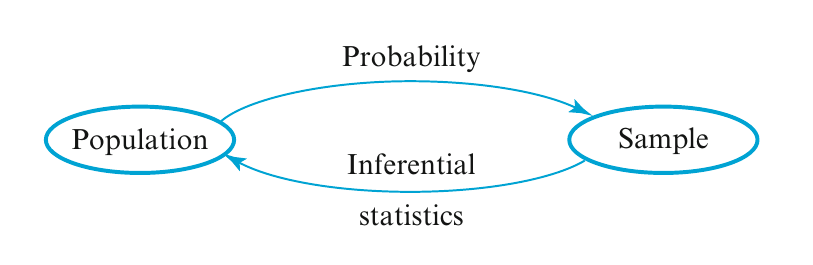
\includegraphics{images/probstat.png}
\caption{}
\end{figure}

Before we can understand what a particular sample can tell us about the
population, we should first understand the uncertainty associated with
taking a sample from a given population. This is why we study
probability before statistics.

\BeginKnitrBlock{example}[Use of manual lap belts in cars equipped with automatic shoulder belt systems]
\protect\hypertarget{ex:unnamed-chunk-6}{}{\label{ex:unnamed-chunk-6}
\iffalse (Use of manual lap belts in cars equipped with automatic
shoulder belt systems) \fi{} }\emph{Probability}: assume that 50\% of
all drivers in a certain metropolitan area regularly use their lap belt
\(\rightarrow\) an assumption about the population. We might ask - How
likely is it that a sample of 100 such drivers will include at least 70
who regularly use their lap belt? - How many of the drivers in a sample
of size 100 can we expect to regularly use their lap belt?

\emph{Inference}: a sample of 100 drivers of such cars revealed that 65
regularly use their lap belt. We might ask\\
- Does this provide substantial evidence for concluding that more than
50\% of all such drivers in this area regularly use their lap belt We
are attempting to use sample information to answer a question about the
structure of the entire population from which the sample was selected.
\EndKnitrBlock{example}

\section{Pictorial and Tabular Methods in Descriptive
Statistics}\label{pictorial-and-tabular-methods-in-descriptive-statistics}

\section{Measures of Location}\label{measures-of-location}

\section{Measures of Variability}\label{measures-of-variability}

\chapter{Probability}\label{probability}

\section*{\texorpdfstring{Introduction\footnote{Reproduced with
  permission from \url{http://www.math.mcgill.ca/dstephens/}}}{Introduction}}\label{introduction1}
\addcontentsline{toc}{section}{Introduction}

The random variation associated with \emph{measurement} procedures in a
scientific analysis requires a framework in which the
\textbf{uncertainty} and \textbf{variability} that are inherent in the
procedure can be handled. The key goal of Probability and Statistical
modelling is to establish a mathematical framework within which
\emph{random} variation (due, for example, to experimental error or
natural variation) can be quantified so that \emph{systematic} variation
(arising due to potentially important biological differences) can be
studied.

Broadly, the \textit{Scientific Process} involves several different
stages:

\begin{equation*}
\begin{array}{cl}
\text{{THEORETICAL MODELLING}} & \rightarrow \text{{MATHEMATICAL/PROBABILISTIC MODELLING}} \\
\downarrow &  \\
\text{{PREDICTION}} &  \\
\downarrow &  \\
\text{{EXPERIMENTATION/OBSERVATION}} &  \\
\downarrow &  \\
\text{{VALIDATION}} &
\end{array}
\end{equation*}

\emph{Mathematical/Probabilistic} \emph{modelling} facilitates
PREDICTION; \emph{Statistical Analysis} provides the means of validation
of predicted behaviour.

To explain the variation in observed data, we need to introduce the
concept of a \emph{probability distribution}. Essentially we need to be
able to model, or specify, or compute the \emph{chance} of observing the
data that we collect or expect to collect. This will then allow us to
assess how likely the data were to occur by chance alone, that is, how
\emph{surprising} the observed data are in light of an assumed
theoretical model.

For example, consider two nucleotide sequences of the same length that
we wish to assess for similarity:

\BeginKnitrBlock{example}[Two nucleotide sequences]
\protect\hypertarget{ex:unnamed-chunk-7}{}{\label{ex:unnamed-chunk-7}
\iffalse (Two nucleotide sequences) \fi{} }

\begin{equation*}
\begin{array}{ll}
\text{{Sequence 1}}{\qquad } & ATAGTAGATACGCACCGAGGA \\
&  \\
\text{{Sequence 2}}{\qquad } & ATCTTAGATAGGCACTGAGGA
\end{array}
\end{equation*}

How can we assess sequence similarity formally ? The number of
discordant positions is 4, but how informative is that summary measure ?
Perhaps we need to assess the chance, for example, that a point mutation
\[ A\rightarrow C \] occurs (as in the discordant position 3) in unit
evolutionary time. Perhaps the chance of observing a sub-sequence

\begin{equation*}
ATCTTA
\end{equation*}

rather than

\begin{equation*}
ATAGTA
\end{equation*}

(in positions 1-6) is important.

\begin{itemize}
\tightlist
\item
  Is the hidden (or \emph{latent}) structure in the sequence,
  corresponding to whether the sequence originates from a coding region
  or otherwise, important ?
\item
  Can we even infer the hidden structure in light of the data we have
  observed ?\\
\end{itemize}
\EndKnitrBlock{example}

These questions can only really be answered when we have an
understanding of randomness and variation. The framework that we will
use to pose and answer such questions formally is given to us by
\emph{probability theory}.

\subsection*{\texorpdfstring{Probability: A Measure of
Uncertainty\footnote{\url{http://www.utstat.toronto.edu/mikevans/jeffrosenthal/book.pdf}}}{Probability: A Measure of Uncertainty}}\label{probability-a-measure-of-uncertainty2}
\addcontentsline{toc}{subsection}{Probability: A Measure of Uncertainty}

Often in life we are confronted by our own ignorance. Whether we are
pondering tonight's traffic jam, tomorrow's weather, next week's stock
prices, an upcoming election, or where we left our hat, often we do not
know an outcome with certainty. Instead, we are forced to guess, to
estimate, to hedge our bets.

\begin{quote}
Probability is the science of uncertainty.
\end{quote}

It provides precise mathematical rules for understanding and analyzing
our own ignorance. It does not tell us tomorrow's weather or next week's
stock prices; rather, it gives us a \textbf{framework for working with
our limited knowledge} and for \textbf{making sensible decisions based
on what we do and do not know}.

To say there is a 40\% chance of rain tomorrow is not to know tomorrow's
weather. Rather, it is to \textbf{know what we do not know} about
tomorrow's weather. In this course, we will develop a more precise
understanding of what it means to say there is a 40\% chance of rain
tomorrow. We will learn how to work with ideas of randomness,
probability, expected value, prediction, estimation, etc., in ways that
are sensible and mathematically clear.

\section{Sample Spaces and Events}\label{sample-spaces-and-events}

\subsection{Sample Spaces}\label{sample-spaces}

\BeginKnitrBlock{definition}[Sample Space]
\protect\hypertarget{def:unnamed-chunk-8}{}{\label{def:unnamed-chunk-8}
\iffalse (Sample Space) \fi{} }The sample space \(\Omega\) is the set of
possible outcomes of an experiment. Points \(\omega\) in \(\Omega\) are
called sample outcomes, realizations, or elements.
\EndKnitrBlock{definition}

\BeginKnitrBlock{example}[Coin tossing]
\protect\hypertarget{ex:unnamed-chunk-9}{}{\label{ex:unnamed-chunk-9}
\iffalse (Coin tossing) \fi{}
}\(\Omega = \left\lbrace H, T \right\rbrace\)
\EndKnitrBlock{example}

\BeginKnitrBlock{example}[Dice]
\protect\hypertarget{ex:unnamed-chunk-10}{}{\label{ex:unnamed-chunk-10}
\iffalse (Dice) \fi{}
}\(\Omega = \left\lbrace 1,2,3,4,5,6 \right\rbrace\)
\EndKnitrBlock{example}

\BeginKnitrBlock{example}[Proportions]
\protect\hypertarget{ex:unnamed-chunk-11}{}{\label{ex:unnamed-chunk-11}
\iffalse (Proportions) \fi{}
}\(\Omega = \left\lbrace x : 0 \leq x \leq 1 \right\rbrace\)
\EndKnitrBlock{example}

\BeginKnitrBlock{example}[Time measurement]
\protect\hypertarget{ex:unnamed-chunk-12}{}{\label{ex:unnamed-chunk-12}
\iffalse (Time measurement) \fi{}
}\(\Omega = \left\lbrace x : x > 0 \right\rbrace = {\mathbb{R}}^{+}\)
\EndKnitrBlock{example}

\BeginKnitrBlock{example}[Temperature measurement]
\protect\hypertarget{ex:unnamed-chunk-13}{}{\label{ex:unnamed-chunk-13}
\iffalse (Temperature measurement) \fi{}
}\(\Omega = \left\{ x:a\leq x\leq b\right\} \subseteq { \mathbb{R}}\)
\EndKnitrBlock{example}

\BeginKnitrBlock{example}[Biological Sequence Analysis]
\protect\hypertarget{ex:unnamed-chunk-14}{}{\label{ex:unnamed-chunk-14}
\iffalse (Biological Sequence Analysis) \fi{} }The experiment may
involve the observation of a nucleotide or protein sequence, so that the
sample space \(\Omega\) may comprise all sequences (of bases/amino
acids) up to a given length, and a sample outcome would be a particular
observed sequence.
\EndKnitrBlock{example}

There are two basic types of experiment: - Counting - Measurement

We shall see that these two types lead to two distinct ways of
specifying probability distributions.

The collection of sample outcomes is a \textbf{set} (a collection of
items) written as

\begin{equation*}
s\in \Omega
\end{equation*}

if \(s\) \emph{is a member of the set} \(\Omega\).

\subsection{Events}\label{events}

\BeginKnitrBlock{definition}[Event]
\protect\hypertarget{def:unnamed-chunk-15}{}{\label{def:unnamed-chunk-15}
\iffalse (Event) \fi{} }An event \(E\) is a subset of the sample space
\(\Omega\) (\(E \subseteq \Omega\)). Events are usually denoted by upper
case letters near the beginning of the alphabet, like \(A, B, C\). An
event which consists of only one outcome is called a simple (or
elementary event); otherwise it is a compound event.
\EndKnitrBlock{definition}

\BeginKnitrBlock{rmdnote}
The sets \(\Omega\) and \(E\) can be either be written as a list of
items, for example,

\begin{equation*}
E=\left\{ s_{1},s_{2},...,s_{n},...\right\}
\end{equation*}

which may a finite or infinite list, or can only be represented by a
continuum of outcomes, for example

\begin{equation*}
E=\left\{ x:0.6<x\leq 2.3\right\}
\end{equation*}
\EndKnitrBlock{rmdnote}

Events are manipulated using \textbf{set theory} notation; if \(A\) and
\(B\) are two events, \(A, B \subseteq \Omega\), then

\begin{itemize}
\tightlist
\item
  \(A \cup B\) is the set of outcomes that belong to \(A\) \textbf{or}
  to \(B\), or to both,
\item
  \(A \cap B\) is the set of outcomes that belong to both \(A\)
  \textbf{and} to \(B\).
\item
  \(A^c\) (complement of \(A\)) is the set of outcomes \textbf{not} in
  \(A\)
\item
  \(A \backslash B = A \cap B^c\)
\end{itemize}

The empty event will be denoted by \(\varnothing\). Two events \(A\) and
\(B\) are mutually exclusive if \(A \cap B = \varnothing\), i.e., the
collection of sample outcomes have no element in common.

\begin{figure}
\centering
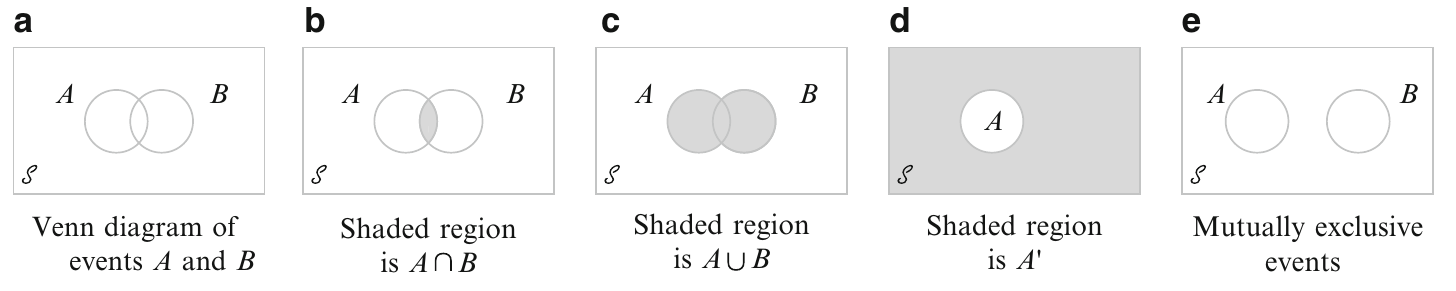
\includegraphics{images/venn.png}
\caption{}
\end{figure}

\section{Axioms, Interpretations, and Properties of
Probability}\label{axioms-interpretations-and-properties-of-probability}

\BeginKnitrBlock{definition}[Axioms (basic properties) of Probability]
\protect\hypertarget{def:unnamed-chunk-17}{}{\label{def:unnamed-chunk-17}
\iffalse (Axioms (basic properties) of Probability) \fi{} }To ensure
that the probability assignments will be consistent with our intuitive
notions of probability, all assign- ments should satisfy the following
axioms (basic properties) of probability

\begin{itemize}
\tightlist
\item
  \textbf{AXIOM 1:} For any event \(A\), \[ P(A) \geq 0 \]
\item
  \textbf{AXIOM 2:} \[ P(\Omega) = 1 \]
\item
  \textbf{AXIOM 3:} If \(A_1, A_2, \ldots\) is an infinite collection of
  disjoint events, then
  \[   P\left(A_1 \cup A_2 \cup \cdots \right) = \sum_{i=1}^{\infty} P(A_i)  \]
\end{itemize}
\EndKnitrBlock{definition}

\BeginKnitrBlock{proposition}
\protect\hypertarget{prp:unnamed-chunk-18}{}{\label{prp:unnamed-chunk-18}}\(P(\varnothing) = 0\)
where \(\varnothing\) is the null event. This in turn implies that the
property contained in Axiom 3 is valid for a finite collection of
events.
\EndKnitrBlock{proposition}

\BeginKnitrBlock{proposition}
\protect\hypertarget{prp:unnamed-chunk-19}{}{\label{prp:unnamed-chunk-19}}For
any event \(A\),\\
\[ P(A) = 1 - P(A^c) \]
\EndKnitrBlock{proposition}

\BeginKnitrBlock{proposition}
\protect\hypertarget{prp:unnamed-chunk-20}{}{\label{prp:unnamed-chunk-20}}For
any event \(A\),\\
\[ P(A) \leq 1 \]
\EndKnitrBlock{proposition}

\BeginKnitrBlock{proposition}
\protect\hypertarget{prp:unnamed-chunk-21}{}{\label{prp:unnamed-chunk-21}}For
any events \(A\) and \(B\),\\
\[ P(A \cup B) = P(A) + P(B) - P(A \cap B) \]
\EndKnitrBlock{proposition}

\section{Counting Techniques}\label{counting-techniques}

When the various outcomes of an experiment are equally likely (the same
probability is assigned to each simple event), the task of computing
probabilities reduces to counting. In particular, if \(N\) is the number
of outcomes in a sample space and \(N(A)\) is the number of outcomes
contained in an event \(A\), then \[ P(A) = \frac{N(A)}{N} \]

\BeginKnitrBlock{proposition}[Product rule for ordered pairs]
\protect\hypertarget{prp:unnamed-chunk-22}{}{\label{prp:unnamed-chunk-22}
\iffalse (Product rule for ordered pairs) \fi{} }If the first element or
object of an ordered pair can be selected in \(n_1\) ways, and for each
of these \(n_1\) ways the second element of the pair can be selected in
\(n_2\) ways, then the number of pairs is \(n_1 \cdot n_2\).
\EndKnitrBlock{proposition}

\subsection{Permutations}\label{permutations}

\BeginKnitrBlock{definition}[Permutation]
\protect\hypertarget{def:unnamed-chunk-23}{}{\label{def:unnamed-chunk-23}
\iffalse (Permutation) \fi{} }Any ordered sequence of \(k\) objects
taken from a set of \(n\) distinct objects is called a permutation of
size \(k\) of the objects. The number of permutations of size \(k\) that
can be constructed from the \(n\) objects is denoted by \(P_k^n\):

\[ P_k^n = \frac{n!}{(n-k)!} \]
\EndKnitrBlock{definition}

\subsection{Combinations}\label{combinations}

\BeginKnitrBlock{definition}[Combination]
\protect\hypertarget{def:unnamed-chunk-24}{}{\label{def:unnamed-chunk-24}
\iffalse (Combination) \fi{} }Given a set of \(n\) distinct objects, any
unordered subset of size \(k\) of the objects is called a combination.
The number of combinations \(n\) of size \(k\) that can be formed from
\(n\) distinct objects will be denoted by

\[ \binom{n}{k} = \frac{n!}{k!(n-k)!} = \frac{P_k^n}{k!} \]
\EndKnitrBlock{definition}

\section{Conditional Probability}\label{conditional-probability}

Conditional probability is the means by which probabilities are updated
in the light of new information. We examine how the information \emph{an
event B has occurred} affects the probability assigned to \(A\).

\BeginKnitrBlock{example}[]
\protect\hypertarget{ex:unnamed-chunk-25}{}{\label{ex:unnamed-chunk-25}
\iffalse () \fi{} }
\EndKnitrBlock{example}

\BeginKnitrBlock{definition}[Conditional Probability]
\protect\hypertarget{def:unnamed-chunk-26}{}{\label{def:unnamed-chunk-26}
\iffalse (Conditional Probability) \fi{} }
\EndKnitrBlock{definition}

\section{Independence}\label{independence}

\appendix


\chapter{Vectorization, *apply and for
loops}\label{vectorization-apply-and-for-loops}

This section will cover the basics of vectorizations, the
\texttt{*apply} family of functions and \texttt{for} loops.

\section{Vectorization}\label{vectorization}

Almost everything in \texttt{R} is a vector. A scalar is really a vector
of length 1 and a \texttt{data.frame} is a collection of vectors. An
nice feature of \texttt{R} is its vectorized capabilities. Vectorization
indicates that a function operates on a whole vector of values at the
same time and not just on a single value\footnote{\url{http://www.dummies.com/how-to/content/how-to-vectorize-your-functions-in-r.html}}.
If you have have ever taken a basic linear algebra course, this concept
will be familiar to you. \newline  \vspace{0.1in} Take for example two
vectors: \newline
\vspace{0.1in} \[
\begin{bmatrix} 1 \\ 2 \\ 3 \end{bmatrix} + 
\begin{bmatrix} 1 \\ 2 \\ 3 \end{bmatrix} =
\begin{bmatrix} 2 \\ 4 \\ 6 \end{bmatrix}
\] \newline  \vspace{0.1in} The corresponding \texttt{R} code is given
by:

\begin{Shaded}
\begin{Highlighting}[]
\NormalTok{a <-}\StringTok{ }\KeywordTok{c}\NormalTok{(}\DecValTok{1}\NormalTok{, }\DecValTok{2}\NormalTok{, }\DecValTok{3}\NormalTok{)}
\NormalTok{b <-}\StringTok{ }\KeywordTok{c}\NormalTok{(}\DecValTok{1}\NormalTok{, }\DecValTok{2}\NormalTok{, }\DecValTok{3}\NormalTok{)}
\NormalTok{a }\OperatorTok{+}\StringTok{ }\NormalTok{b}
\end{Highlighting}
\end{Shaded}

\begin{verbatim}
## [1] 2 4 6
\end{verbatim}

Many of the \texttt{base} functions in \texttt{R} are already
vectorized. Here are some common examples:

\begin{Shaded}
\begin{Highlighting}[]
\CommentTok{# generate a sequence of numbers from 1 to 10}
\NormalTok{(a <-}\StringTok{ }\DecValTok{1}\OperatorTok{:}\DecValTok{10}\NormalTok{)}
\end{Highlighting}
\end{Shaded}

\begin{verbatim}
##  [1]  1  2  3  4  5  6  7  8  9 10
\end{verbatim}

\begin{Shaded}
\begin{Highlighting}[]
\CommentTok{# sum the numbers from 1 to 10}
\KeywordTok{sum}\NormalTok{(a)}
\end{Highlighting}
\end{Shaded}

\begin{verbatim}
## [1] 55
\end{verbatim}

\begin{Shaded}
\begin{Highlighting}[]
\CommentTok{# calculate sums of each column}
\KeywordTok{colSums}\NormalTok{(iris[, }\OperatorTok{-}\DecValTok{5}\NormalTok{])}
\end{Highlighting}
\end{Shaded}

\begin{verbatim}
## Sepal.Length  Sepal.Width Petal.Length  Petal.Width 
##        876.5        458.6        563.7        179.9
\end{verbatim}

\begin{quote}
\textbf{Exercise}: What happens when you sum two vectors of different
lengths?
\end{quote}

\section{\texorpdfstring{Family of \texttt{*apply}
functions}{Family of *apply functions}}\label{family-of-apply-functions}

\begin{itemize}
\tightlist
\item
  \texttt{apply}, \texttt{lapply} and \texttt{sapply} are some of the
  most commonly used class of functions in \texttt{R}
\item
  \texttt{*apply} functions are not necessarily faster than loops, but
  can be easier to read (and vice cersa)
\item
  \texttt{apply} is used when you need to perform an operation on every
  row or column of a matrix or data.frame
\item
  \texttt{lapply} and \texttt{sapply} differ in the format of the
  output. The former returns a list while the ladder returns a vector
\item
  There are other \texttt{*apply} functions such as \texttt{tapply},
  \texttt{vapply} and \texttt{mapply} with similar functionality and
  purpose
\end{itemize}

\subsection{Loops vs.~Apply}\label{loops-vs.apply}

\begin{Shaded}
\begin{Highlighting}[]
\CommentTok{# Getting the row means of two columns Generate data}
\NormalTok{N <-}\StringTok{ }\DecValTok{10000}
\NormalTok{x1 <-}\StringTok{ }\KeywordTok{runif}\NormalTok{(N)}
\NormalTok{x2 <-}\StringTok{ }\KeywordTok{runif}\NormalTok{(N)}
\NormalTok{d <-}\StringTok{ }\KeywordTok{as.data.frame}\NormalTok{(}\KeywordTok{cbind}\NormalTok{(x1, x2))}
\KeywordTok{head}\NormalTok{(d)}
\end{Highlighting}
\end{Shaded}

\begin{verbatim}
##           x1         x2
## 1 0.64870088 0.74703487
## 2 0.33200087 0.35791966
## 3 0.01155646 0.84240065
## 4 0.81397243 0.18195049
## 5 0.49752317 0.09354495
## 6 0.04255033 0.41102094
\end{verbatim}

\begin{Shaded}
\begin{Highlighting}[]
\CommentTok{# Loop: create a vector to store the results in}
\NormalTok{rowMeanFor <-}\StringTok{ }\KeywordTok{vector}\NormalTok{(}\StringTok{"double"}\NormalTok{, N)}

\ControlFlowTok{for}\NormalTok{ (i }\ControlFlowTok{in} \KeywordTok{seq_len}\NormalTok{(N)) \{}
\NormalTok{    rowMeanFor[[i]] <-}\StringTok{ }\KeywordTok{mean}\NormalTok{(}\KeywordTok{c}\NormalTok{(d[i, }\DecValTok{1}\NormalTok{], d[i, }\DecValTok{2}\NormalTok{]))}
\NormalTok{\}}

\CommentTok{# Apply:}
\NormalTok{rowMeanApply <-}\StringTok{ }\KeywordTok{apply}\NormalTok{(d, }\DecValTok{1}\NormalTok{, mean)}

\CommentTok{# are the results equal}
\KeywordTok{all.equal}\NormalTok{(rowMeanFor, rowMeanApply)}
\end{Highlighting}
\end{Shaded}

\begin{verbatim}
## [1] TRUE
\end{verbatim}

\subsection{\texorpdfstring{Descriptive Statistics using
\texttt{*apply}}{Descriptive Statistics using *apply}}\label{descriptive-statistics-using-apply}

\begin{Shaded}
\begin{Highlighting}[]
\KeywordTok{data}\NormalTok{(women)}
\CommentTok{# data structure}
\KeywordTok{str}\NormalTok{(women)}
\end{Highlighting}
\end{Shaded}

\begin{verbatim}
## 'data.frame':    15 obs. of  2 variables:
##  $ height: num  58 59 60 61 62 63 64 65 66 67 ...
##  $ weight: num  115 117 120 123 126 129 132 135 139 142 ...
\end{verbatim}

\begin{Shaded}
\begin{Highlighting}[]
\CommentTok{# calculate the mean for each column}
\KeywordTok{apply}\NormalTok{(women, }\DecValTok{2}\NormalTok{, mean)}
\end{Highlighting}
\end{Shaded}

\begin{verbatim}
##   height   weight 
##  65.0000 136.7333
\end{verbatim}

\begin{Shaded}
\begin{Highlighting}[]
\CommentTok{# apply 'fivenum' function to each column}
\KeywordTok{vapply}\NormalTok{(women, fivenum, }\KeywordTok{c}\NormalTok{(}\DataTypeTok{Min. =} \DecValTok{0}\NormalTok{, }\StringTok{`}\DataTypeTok{1st Qu.}\StringTok{`}\NormalTok{ =}\StringTok{ }\DecValTok{0}\NormalTok{, }\DataTypeTok{Median =} \DecValTok{0}\NormalTok{, }\StringTok{`}\DataTypeTok{3rd Qu.}\StringTok{`}\NormalTok{ =}\StringTok{ }\DecValTok{0}\NormalTok{, }
    \DataTypeTok{Max. =} \DecValTok{0}\NormalTok{))}
\end{Highlighting}
\end{Shaded}

\begin{verbatim}
##         height weight
## Min.      58.0  115.0
## 1st Qu.   61.5  124.5
## Median    65.0  135.0
## 3rd Qu.   68.5  148.0
## Max.      72.0  164.0
\end{verbatim}

\subsection{\texorpdfstring{Creating new columns using
\texttt{sapply}}{Creating new columns using sapply}}\label{creating-new-columns-using-sapply}

You can apply a \emph{user defined function} to columns or the entire
data frame:

\begin{Shaded}
\begin{Highlighting}[]
\CommentTok{# the ouput of sapply is a vector the 's' in sapply stands for 'simplified'}
\CommentTok{# apply}
\NormalTok{mtcars}\OperatorTok{$}\NormalTok{gear2 <-}\StringTok{ }\KeywordTok{sapply}\NormalTok{(mtcars}\OperatorTok{$}\NormalTok{gear, }\ControlFlowTok{function}\NormalTok{(i) }\ControlFlowTok{if}\NormalTok{ (i }\OperatorTok{==}\StringTok{ }\DecValTok{4}\NormalTok{) }\StringTok{"alot"} \ControlFlowTok{else} \StringTok{"some"}\NormalTok{)}

\KeywordTok{head}\NormalTok{(mtcars)[, }\KeywordTok{c}\NormalTok{(}\StringTok{"gear"}\NormalTok{, }\StringTok{"gear2"}\NormalTok{)]}
\end{Highlighting}
\end{Shaded}

\begin{verbatim}
##                   gear gear2
## Mazda RX4            4  alot
## Mazda RX4 Wag        4  alot
## Datsun 710           4  alot
## Hornet 4 Drive       3  some
## Hornet Sportabout    3  some
## Valiant              3  some
\end{verbatim}

\subsection{\texorpdfstring{Applying functions to subsets using
\texttt{tapply}}{Applying functions to subsets using tapply}}\label{applying-functions-to-subsets-using-tapply}

\begin{Shaded}
\begin{Highlighting}[]
\CommentTok{# Fisher's famous dataset}
\KeywordTok{data}\NormalTok{(iris)}
\KeywordTok{str}\NormalTok{(iris)}
\end{Highlighting}
\end{Shaded}

\begin{verbatim}
## 'data.frame':    150 obs. of  5 variables:
##  $ Sepal.Length: num  5.1 4.9 4.7 4.6 5 5.4 4.6 5 4.4 4.9 ...
##  $ Sepal.Width : num  3.5 3 3.2 3.1 3.6 3.9 3.4 3.4 2.9 3.1 ...
##  $ Petal.Length: num  1.4 1.4 1.3 1.5 1.4 1.7 1.4 1.5 1.4 1.5 ...
##  $ Petal.Width : num  0.2 0.2 0.2 0.2 0.2 0.4 0.3 0.2 0.2 0.1 ...
##  $ Species     : Factor w/ 3 levels "setosa","versicolor",..: 1 1 1 1 1 1 1 1 1 1 ...
\end{verbatim}

\begin{Shaded}
\begin{Highlighting}[]
\CommentTok{# mean sepal length by species}
\KeywordTok{tapply}\NormalTok{(iris}\OperatorTok{$}\NormalTok{Sepal.Length, iris}\OperatorTok{$}\NormalTok{Species, mean)}
\end{Highlighting}
\end{Shaded}

\begin{verbatim}
##     setosa versicolor  virginica 
##      5.006      5.936      6.588
\end{verbatim}

\subsection{\texorpdfstring{Nested for loops using
\texttt{mapply}}{Nested for loops using mapply}}\label{nested-for-loops-using-mapply}

\texttt{mapply} is my favorite \texttt{base} \texttt{R} function and
here are some reasons why:

\begin{itemize}
\tightlist
\item
  Using \texttt{mapply} is equivalent to writing nested \texttt{for}
  loops except that it is 100\% more human readable and less prone to
  errors
\item
  It is an effective way of conducting simulations because it iterates
  of many arguments
\end{itemize}

Let's say you want to generate random samples from a normal distribution
with varying means and standard deviations. Of course the brute force
way would be to write out the command once, copy paste as many times as
you want, and then manually change the arguments for \texttt{mean} and
\texttt{sd} in the \texttt{rnorm} function as so:

\begin{Shaded}
\begin{Highlighting}[]
\NormalTok{v1 <-}\StringTok{ }\KeywordTok{rnorm}\NormalTok{(}\DecValTok{100}\NormalTok{, }\DataTypeTok{mean =} \DecValTok{5}\NormalTok{, }\DataTypeTok{sd =} \DecValTok{1}\NormalTok{)}
\NormalTok{v2 <-}\StringTok{ }\KeywordTok{rnorm}\NormalTok{(}\DecValTok{100}\NormalTok{, }\DataTypeTok{mean =} \DecValTok{10}\NormalTok{, }\DataTypeTok{sd =} \DecValTok{5}\NormalTok{)}
\NormalTok{v3 <-}\StringTok{ }\KeywordTok{rnorm}\NormalTok{(}\DecValTok{100}\NormalTok{, }\DataTypeTok{mean =} \OperatorTok{-}\DecValTok{3}\NormalTok{, }\DataTypeTok{sd =} \DecValTok{10}\NormalTok{)}
\end{Highlighting}
\end{Shaded}

This isn't too bad for three vectors. But what if you want to generate
many more combinations of means and sds ? Furthermore, how can you keep
track of the parameters you used? Now lets consider the \texttt{mapply}
function:

\begin{Shaded}
\begin{Highlighting}[]
\NormalTok{means <-}\StringTok{ }\KeywordTok{c}\NormalTok{(}\DecValTok{5}\NormalTok{, }\DecValTok{10}\NormalTok{, }\OperatorTok{-}\DecValTok{3}\NormalTok{)}
\NormalTok{sds <-}\StringTok{ }\KeywordTok{c}\NormalTok{(}\DecValTok{1}\NormalTok{, }\DecValTok{5}\NormalTok{, }\DecValTok{10}\NormalTok{)}

\CommentTok{# MoreArgs is a list of arguments that dont change}
\NormalTok{randomNormals <-}\StringTok{ }\KeywordTok{mapply}\NormalTok{(rnorm, }\DataTypeTok{mean =}\NormalTok{ means, }\DataTypeTok{sd =}\NormalTok{ sds, }\DataTypeTok{MoreArgs =} \KeywordTok{list}\NormalTok{(}\DataTypeTok{n =} \DecValTok{100}\NormalTok{))}

\KeywordTok{head}\NormalTok{(randomNormals)}
\end{Highlighting}
\end{Shaded}

\begin{verbatim}
##          [,1]      [,2]       [,3]
## [1,] 5.268941 15.241578  -7.939710
## [2,] 5.534837  6.284061  -8.965358
## [3,] 3.988739  6.987539   9.444327
## [4,] 5.767137 10.381598 -17.553147
## [5,] 6.728720  2.503015  22.107234
## [6,] 5.056595  6.401967   8.257844
\end{verbatim}

The following diagram (from
\href{http://r4ds.had.co.nz/iteration.html\#mapping-over-multiple-arguments}{r4ds})
describes exactly what is going on in the above function call to
\texttt{mapply}:

\begin{figure}
\centering
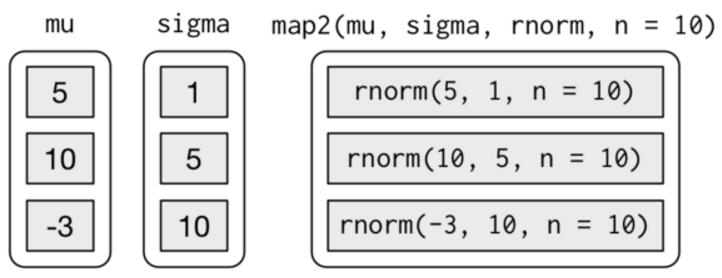
\includegraphics{images/mapply.png}
\caption{}
\end{figure}

Advantages:

\begin{enumerate}
\def\labelenumi{\arabic{enumi}.}
\tightlist
\item
  Result is automatically stored in a matrix
\item
  The parameters are also saved in \texttt{R} objects so that they can
  be easily manipulated and/or recovered
\end{enumerate}

Consider a more complex scenario where you want to consider many
possible combinations of means and sds. We take advantage of the
\texttt{expand.grid} function to create a \texttt{data.frame} of
simulation parameters:

\begin{Shaded}
\begin{Highlighting}[]
\NormalTok{simParams <-}\StringTok{ }\KeywordTok{expand.grid}\NormalTok{(}\DataTypeTok{means =} \DecValTok{1}\OperatorTok{:}\DecValTok{10}\NormalTok{, }\DataTypeTok{sds =} \DecValTok{1}\OperatorTok{:}\DecValTok{10}\NormalTok{)}

\NormalTok{randomNormals <-}\StringTok{ }\KeywordTok{mapply}\NormalTok{(rnorm, }\DataTypeTok{mean =}\NormalTok{ simParams}\OperatorTok{$}\NormalTok{means, }\DataTypeTok{sd =}\NormalTok{ simParams}\OperatorTok{$}\NormalTok{sds, }\DataTypeTok{MoreArgs =} \KeywordTok{list}\NormalTok{(}\DataTypeTok{n =} \DecValTok{100}\NormalTok{))}

\KeywordTok{dim}\NormalTok{(randomNormals)}
\end{Highlighting}
\end{Shaded}

\begin{verbatim}
## [1] 100 100
\end{verbatim}

\section{\texorpdfstring{Creating dynamic documents with
\texttt{mapply}}{Creating dynamic documents with mapply}}\label{creating-dynamic-documents-with-mapply}

\texttt{mapply} together with the \texttt{rmarkdown} package
\citep{R-rmarkdown} can be very useful to create dynamic documents for
exploratory analysis. We illustrate this using the Motor Trend Car Road
Tests data which comes pre-loaded in \texttt{R}.

\begin{quote}
The data was extracted from the 1974 Motor Trend US magazine, and
comprises fuel consumption and 10 aspects of automobile design and
performance for 32 automobiles (1973--74 models).
\end{quote}

Copy the code below in a file called \texttt{mapplyRmarkdown.Rmd} :

Copy the code below in a file called \texttt{boxplotTemplate} :

\chapter{Appendix B}\label{appendix-b}

\bibliography{packages.bib,book.bib}


\end{document}
